\chapter{Systemarkitektur}

\subsection{Domæne model}
På figur \ref{fig:DomainModel} ses domæne modellen for systemet. Denne er udarbejdet ved at lave en navneordsanalyse fra de use cases der er specificerede i afsnit \ref{afsnit:kravspecifikation}.

\begin{figure}[H]
	\centering
	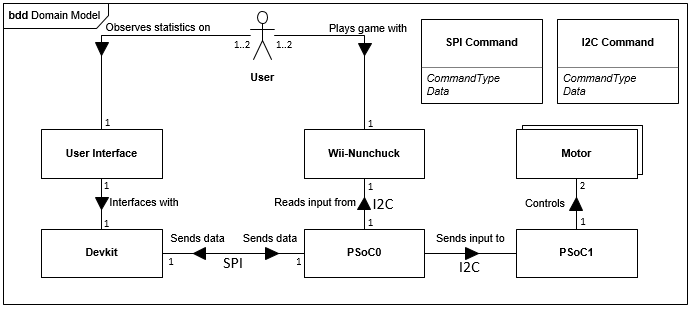
\includegraphics[width=\textwidth]{Systemarkitektur/images/DomainModel}
	\caption{Domæne model for systemet}
	\label{fig:DomainModel}
\end{figure}

I domæne modellen ses det, at brugeren interagerer med både Wii-nunchucken og med brugergrænsefladen. Brugergrænsefladen er en grænseflade til devkittet. Devkittet kommunikerer med PSoC0, som læser den analoge data der kommer fra Wii-nunchucken. Denne data bliver derefter afkodet og videresendt til PSoC1, som ud fra denne data styrer de forskellige motorer.

% ---------------BDD--------------------------------------------------
\subsection{BDD for Candygun 3000}
I BDD-diagrammet på figur \ref{fig:BDD} er Candygun 3000 brudt ned i blokkene PSoC0, PSoC1, PSoC2 og Devkit 8000. Devkit 8000 er brugergrænsefladen, som brugeren kan interagere med via touchskærmen. Den er forbundet via SPI til PSoC0, som er SPI-slave. PSoC0 er desuden også I2C-master. PSoC0 kommunikerer via I2C til PSoC1 og PSoC2. PSoC1 står for motorstyring, som via et PWM-signal styrer de 3 motorer. PSoC2 har til opgave at aflæse brugerinput fra Wii-nunchucken, som også kommunikerer via I2C. På figur \ref{fig:BDD} ses de forskellige blokke og deres porte. Desuden er der en flowspecification for I2C og SPI, hvor forbindelserne er beskrevet mere detaljeret (set fra master-synspunkt). 

\begin{figure}[H]
	\centering
	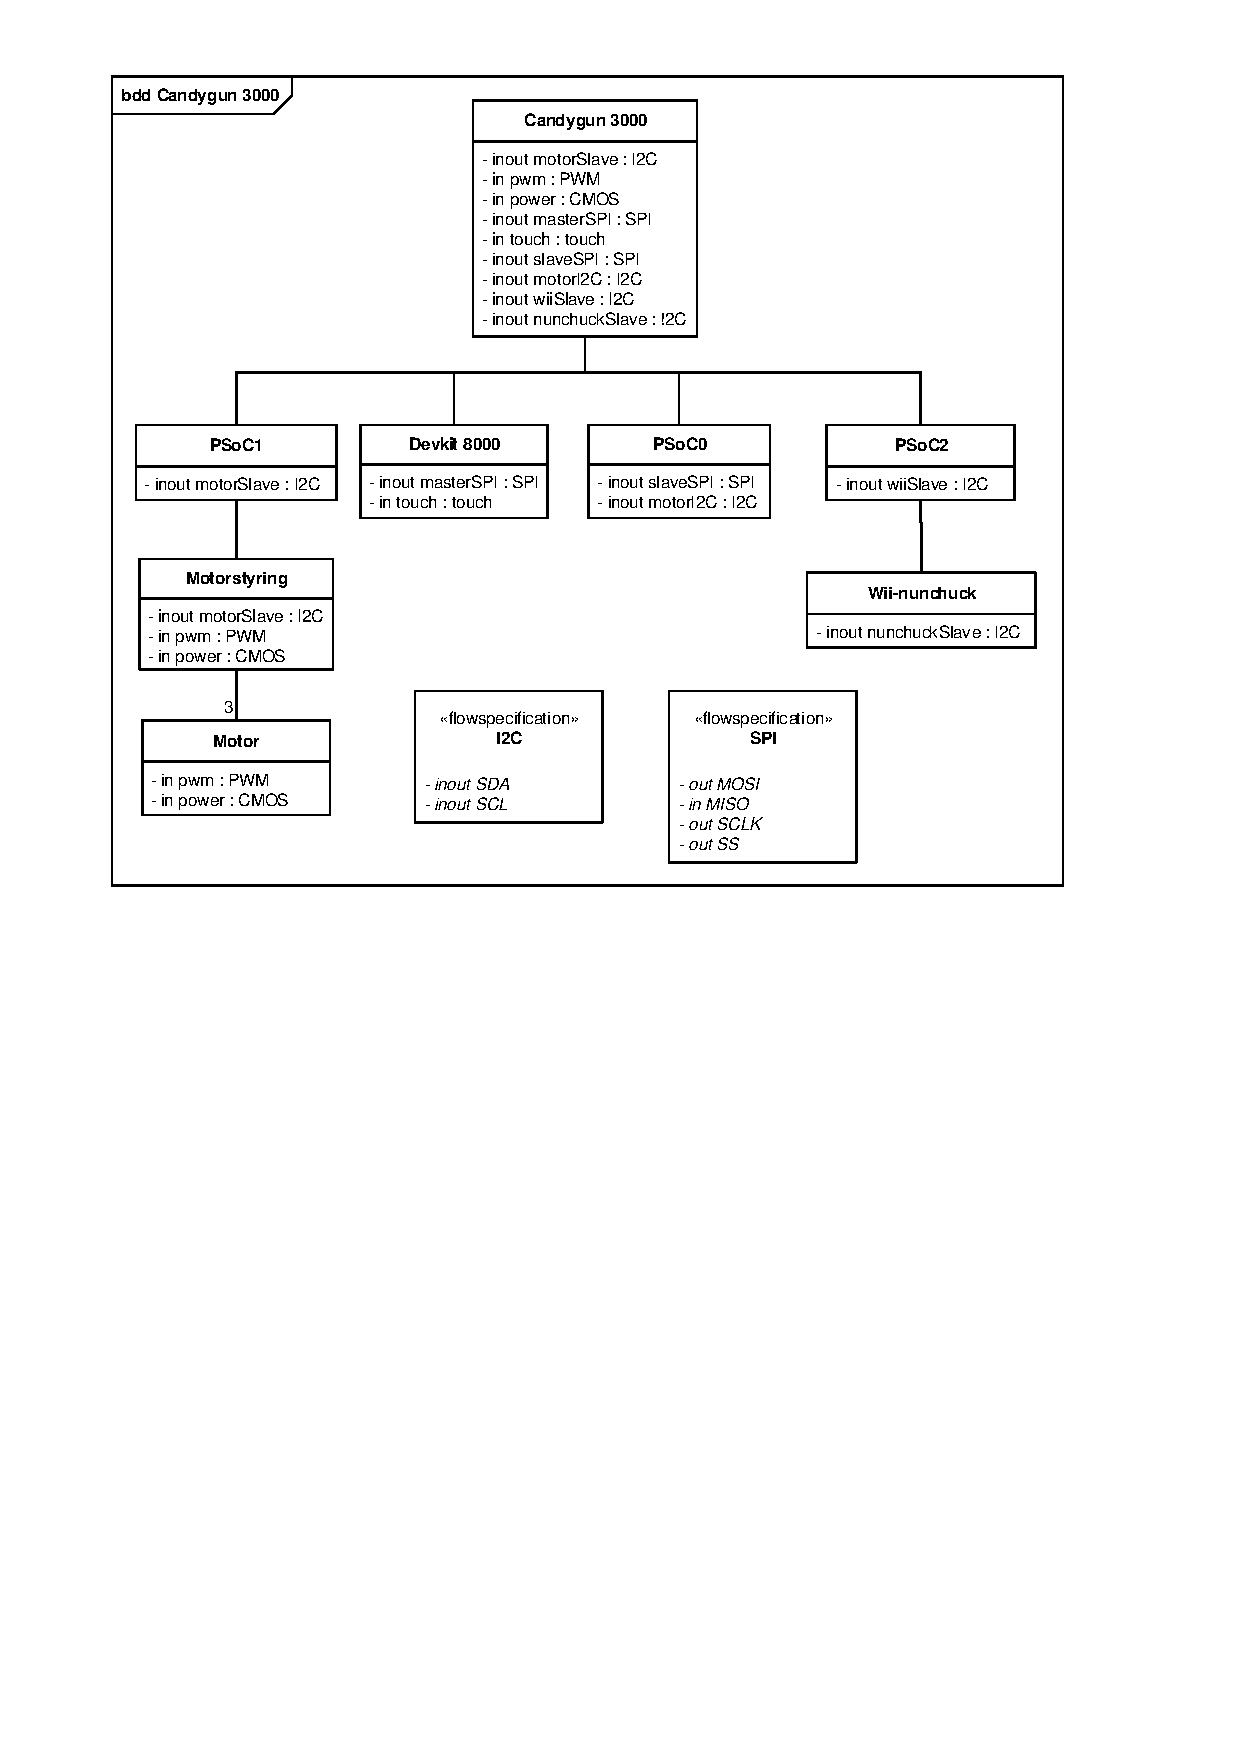
\includegraphics[trim = {1.8cm 14.6cm 1.8cm 1cm}, clip = true, width = \textwidth]{Systemarkitektur/images/BDD_overordnet.pdf}
	\caption{Overordnet BDD for Candygun 3000.}
	\label{fig:BDD}
\end{figure}


\subsubsection{Blokbeskrivelse}
\textbf{DevKit 8000}
\newline
\textit{DevKit 8000} er en embedded Linux platform med touch-skærm der bruges til brugergrænsefladen for produktet. Det er her hvor brugeren interagerer med systemet og ser status for spillet.

\textbf{Motorstyring}
\newline
\textit{Motorstyring} er blokken som består af Candy Gun 3000's motorerer - brugt til at styre den - samt \textit{PSoC1}, som bruges til styring af disse motorer.

\textbf{Wii-Nunchuck-Styring}

\textit{Wii-Nunchuck-Styring} er blokken som består af den fysiske Wii-Nunchuck controller der bruges af brugeren til at styre kanonen, samt \textit{PSoC2}, som bruges til at videresende I2C dataen fra controlleren.

\textbf{Wii-Nunchuck}

\textit{Wii-Nunchuck} er controlleren brugeren styrer kanonen med.

\textbf{Motor}

\textit{Motor} blokken er Candy Gun 3000's motorerer der bruges til styring af kanonen i forskellige retninger.

\textbf{PSoC0}

\textit{PSoC0} er PSoC hardware der både er I2C master og SPI slave. Denne PSoC fungerer som bindeled mellem resten af systemets hardware, så kommunikation er muligt.

\textbf{PSoC1}

\textit{PSoC1} er PSoC hardware der bruges til softwarestyring af Candy Gun 3000's motorerer samt affyringsmekanisme.

\textbf{PSoC2}

\textit{PSoC2} er PSoC hardware der bruges til at videresende input data fra Wii-Nunchuck controlleren.	

\textbf{SPI (FlowSpecification)}

\textit{SPI (FlowSpecification)} beskriver signalerne der indgår i \textit{SPI} kommunikation.

\textbf{I2C (FlowSpecification)}

\textit{I2C (FlowSpecification)} beskriver signalerne der indgår i \textit{I2C} kommunikation.
% ---------------IBD--------------------------------------------------
\subsection{IBD for Candygun 3000}
I IBD'et på figur \ref{fig:IBD} er forbindelserne mellem de forskellige blokke overskueliggjort. Det er dermed let at få et overblik over, hvilke grænseflader der skal tages højde for i den videre udvikling. 

\begin{figure}[H]
	\centering
	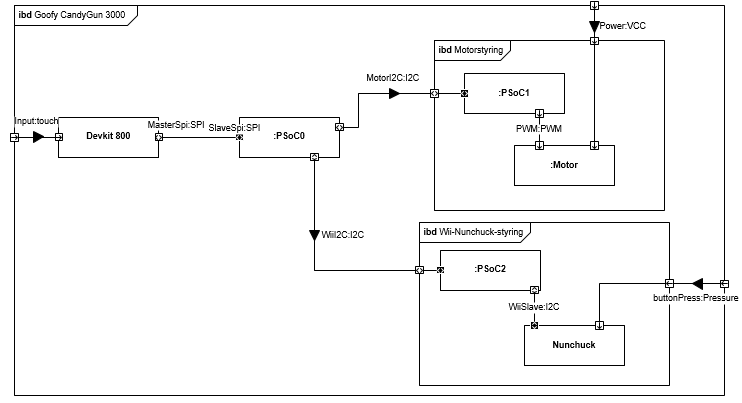
\includegraphics[width=\textwidth]{Systemarkitektur/images/GoofycandygunIBD.png}
	\caption{IBD for Candygun 3000}
	\label{fig:IBD}
\end{figure}

\subsubsection{Signalbeskrivelse}
Generelt for signalbeskrivelsen gælder, at når et signal beskrives som 'højt' menes der i et spændingsområde på 3.5V til 5 V, som er defineret for CMOS kredse \cite{cmosStandard}. På samme måde er signaler beskrevet som 'lav' defineret som spændinger indenfor 0 V til 1.5 V.
\begin{longtable}{|>{\hspace{0pt}}p{3cm} | >{\hspace{0pt}}p{3cm} | p{2cm} | p{3cm} |}
	\hline
	\textbf{Blok-navn} & \textbf{Funktionsbeskrivelse} & \textbf{Signaler} & \textbf{Signalbeskrivelse} \\ \hline
	Devkit8000 & Fungerer som grænseflade mellem bruger og systemet. & masterSPI & Type: SPI \newline Spændingsniveau: 0-5V \newline Hastighed: ?? \\ \cline{3-4}
	& & touch & Type: touch \newline Tryk på DevKit8000 display. \\ \hline
	PSoC0 & Fungerer som I2C master for systemet samt SPI slave til DevKit8000. & slaveSPI & Type: SPI \newline Spændingsniveau: 0-5V \newline Hastighed: ?? \\ \cline{3-4}
	& & masterI2C & Type: I2C \newline Spændingsniveau: 0-5V \newline Hastighed: 100kbit/sekund \\ \hline
	Motorstyring & Modtager input fra Wii-Nunchuck og omsætter det til PWM signaler. & motorSlave & Type: I2C \newline Spændingsniveau: 0-5V \newline Hastighed: 100kbit/sekund \newline Beskrivelse: Indeholder Wii-Nunchuck data der skal bruges til motorstyring.  \\ \cline{3-4}
	& & power & Type: \(V_{CC}\) \newline Spændingsniveau: 5V \newline Beskrivelse: Strømforsyning til motorstyringen. \\ \hline
	PSoC1 & Modtager input fra Wii-Nunchuck og omsætter det til PWM signaler. & MotorI2C & Type: I2C \newline Spændingsniveau: 0-5V \newline Hastighed: 100kbit/sekund \newline Beskrivelse: Indeholder formatteret Wii-Nunchuck data som skal bruges til styring af motorens PWM signal. \\ \cline{3-4} 
	& & PWM & Type: PWM \newline Frekvens: 22kHz \newline PWM \%: 0-100\% \newline Spændingsniveau: 0-5V \newline Beskrivelse: PWM signal til styring af motorens hastighed. Udregnet ud fra MotorI2C signalet. \\ \hline
	Motor & Motorerne der skal styre kanonen & PWM & Type: PWM \newline Frekvens: 22kHz \newline PWM\%: 0-100\% \newline Spædingsniveau: 0-5V \newline Beskrivelse: PWM signal til styring af motorens hastighed. \\ \cline{3-4}
	& & power & Type: \(V_{CC}\) \newline Spændingsniveau: 12V \newline Beskrivelse: Strømforsyning til motorstyringen  \\ \hline
	PSoC2 & Modtager input data fra Wii-Nunchuk og videresender det i behandlet format. & wiiSlave & Type: I2C \newline Spændingsniveau: 0-5V \newline Hastighed: 100kbit/sekund \newline Beskrivelse: Sender input data fra Wii-Nunchuck til PSoC2. \\ \cline{3-4}
	& & WiiI2C & Type: I2C \newline Spændingsniveau: 0-5V \newline Hastighed: 100kbit/sekund \newline Beskrivelse: Videresender behandlet Wii-Nunchuk data til andre dele af systemet. \\ \hline
	Wii-nunchuck & Den fysiske controller som brugeren styrer kanonen med. & WiiSlave & Type: I2C \newline Spændingsniveau: 0-5V \newline Hastighed: 100kbit/sekund \newline Beskrivelse: Denne I2C linje bruges til kommunikation mellem PSoC 2 og Wii-Nunchuck. \\ \cline{3-4}
	& & buttonPress & Type: I2C \newline Det fysiske tryk når brugeren trykker på Wii-Nunchuck knapper. \\ \hline
	SPI & Denne blok beskriver den ikke-atomiske SPI forbindelse. & MOSI & Type: CMOS \ Spændingsniveau: 0-5V \newline Hastighed: ?? \newline Beskrivelse: Binært data som sendes fra master til slave. \\ \cline{3-4}
	& & MISO & Type: CMOS \newline Spændingsniveau: 0-5V \newline Hastighed: ?? \newline Beskrivelse: Binært data som sendes fra slave til master. \\ \cline{3-4}
	& & SCLK & Type: CMOS \newline Spændingsniveau: 0-5V \newline Hastighed: ?? \newline Beskrivelse: Clock signalet fra master til slave, som bruges til at synkronisere den serielle kommunikation. \\ \cline{3-4}
	& & SS & Type: CMOS \newline Spændingsniveau: 0-5V \newline Hastighed: ?? \newline  Beskrivelse: Slave-Select, som bruges til at vælge slaven der skal modtage og sende data. \\ \hline
	I2C & Denne blok beskriver den ikke-atomiske I2C forbindelse. & SDA & Type: CMOS \newline Spændingsniveau: 0-5V \newline Hastighed: ?? \newline Beskrivelse: Databussen mellem I2C masteren og I2C slaver. \\ \cline{3-4}
	& & SCL & Type: CMOS \newline Spændingsniveau: 0-5V \newline Hastighed: ?? \newline Beskrivelse: Clock signalet fra master til lyttende I2C slaver, som bruges til at synkronisere den serielle kommunikation. \\ \hline
\end{longtable}

\section{Hardware Arkitektur}
I hardwarearkitekturen brydes systemet ned i dele, som senere gør det muligt at uddele arbejdsopgaver, og specificere grænseflader. Hardwarearkitekturen består at BDD og IBD for systemet.

\section{Software Arkitektur}
I softwarearkitekturen udarbejdes der applikationsmodeller bestående af sekvensdiagrammer og klassediagrammer for hvert delsystem. Denne arkitektur overskueliggører kravene til de boundaryklasser, der muliggør kommunikation mellem delsystemerne. Derudover bliver der gennem analyse af use case og sekvensdiagrammer udledt grundlæggende metoder i klasserne.  

% ---------------Devkit Applikationsmodel-----------------------------
\subsection{Applikationsmodel for Devkit 8000}
Sekvensdiagrammet for Devkit 8000 ses på figur \ref{fig:sekvensDevkit}. Der tages udgangspunkt i use case 2. Der er to boundaryklasser, da brugergrænsefladen skal håndtere kommunikationen mellem brugeren og PSoC0. Brugeren interagerer via en grafisk brugergrænseflade (GUI). Boundaryklassen ComProtocol, skal håndtere SPI-kommunikationen til PSoC0. Som det ses af diagrammet initieres testen af brugeren og derefter er det kontrolklassen, der sørger for, at de forskellige tests bliver sat i gang. Når en test er færdiggjort meldes resultatet ud til brugeren via GUI'en.

\begin{figure}[H]
	\centering
	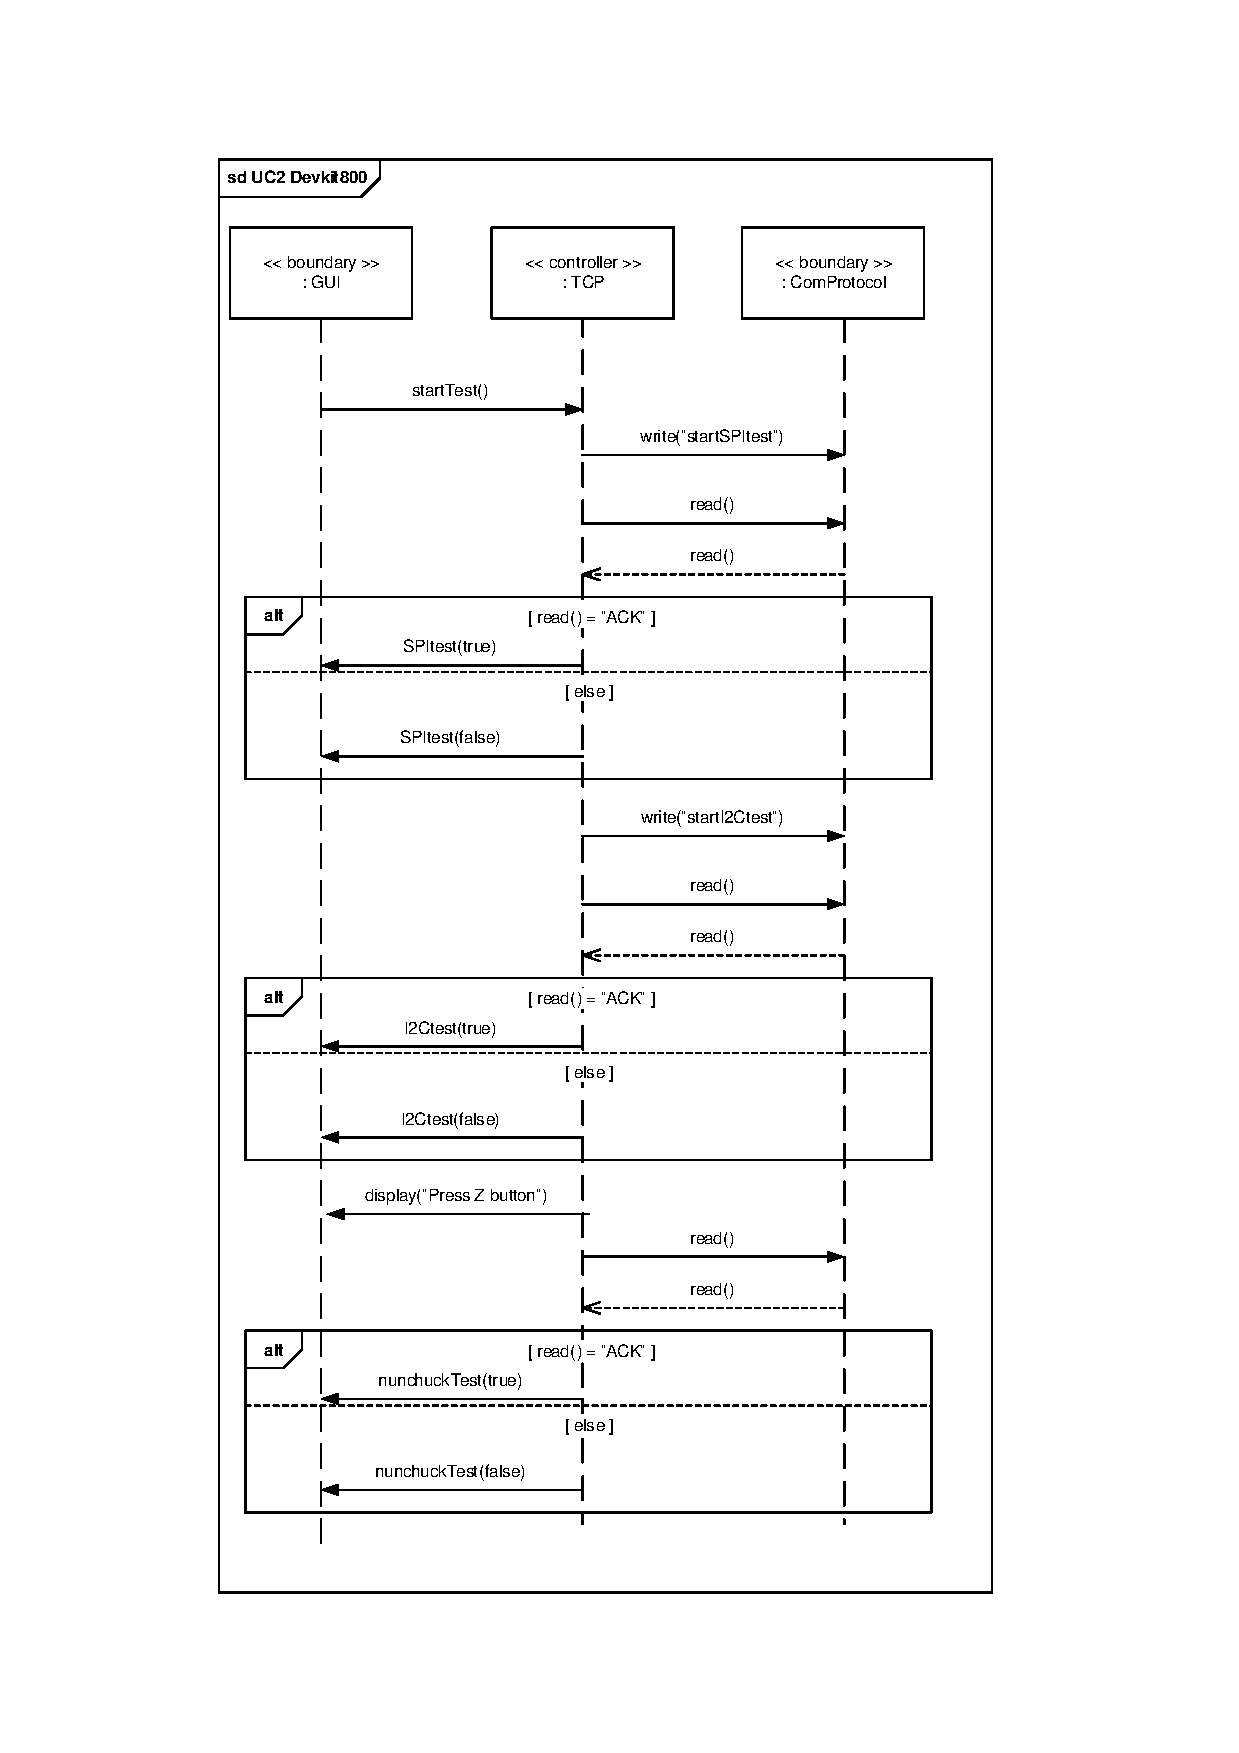
\includegraphics[trim = {3.6cm 2.7cm 4cm 2.7cm}, clip = true, width=\textwidth] {Systemarkitektur/images/SekvensdiagramDevkit.pdf}
	\caption{Sekvensdiagram for Devkit 8000}
	\label{fig:sekvensDevkit}
\end{figure}
Ud fra sekvensdiagrammet for Devkit 8000 er der udledt disse metoder til klasserne. De ses i klassediagrammet på figur \ref{fig:klasseDevkit}. 

\begin{figure}[H]
	\centering
	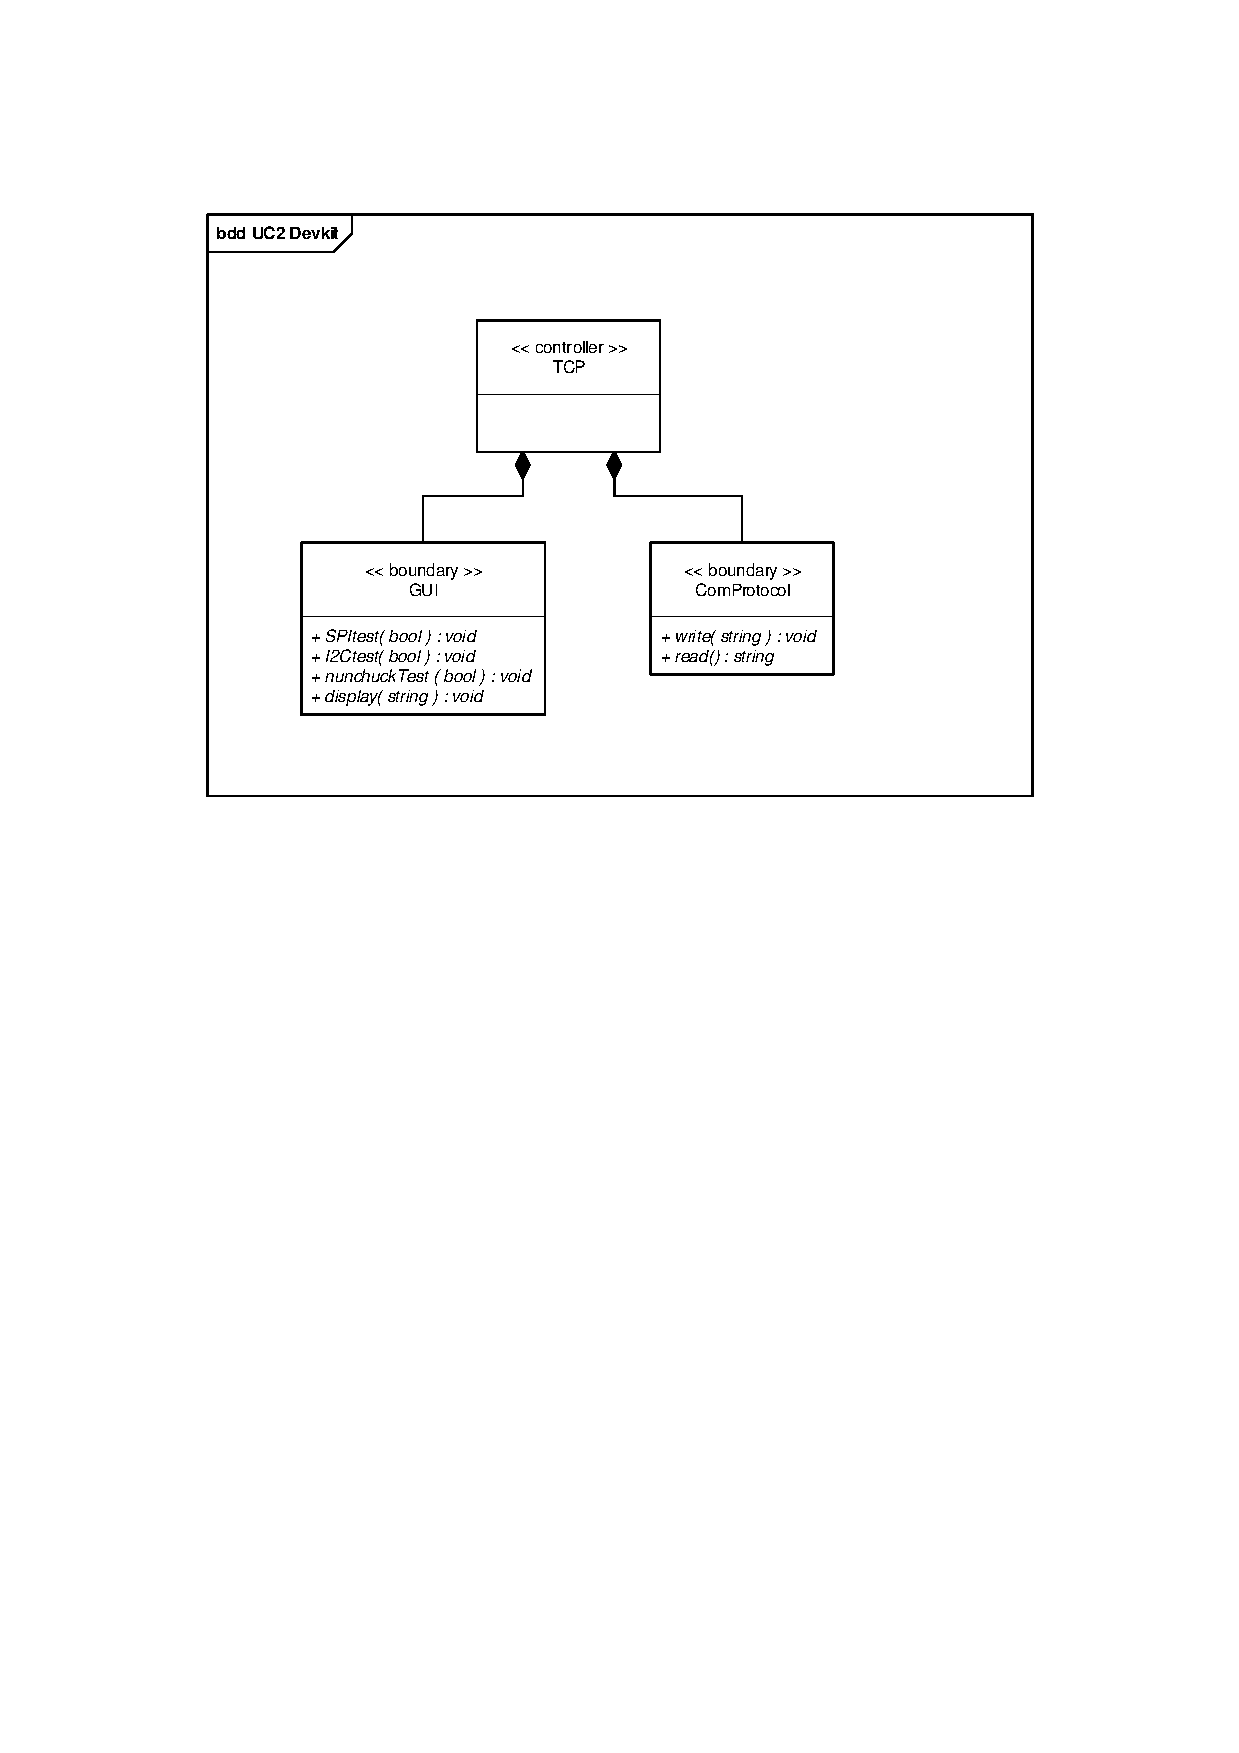
\includegraphics[trim = {3.2cm 16.1cm 3.2cm 3.5cm}, clip = true, width=\textwidth] {Systemarkitektur/images/klassediagramDevkit.pdf}
	\caption{Klassediagram for Devkit 8000}
	\label{fig:klasseDevkit}
\end{figure}

% ---------------PSoC0 Applikationsmodel-----------------------------
\subsection{Applikationsmodel for PSoC0}
På figur \ref{fig:sekvensPSoC0SPITest}, \ref{fig:sekvensPSoC0I2CTest} og \ref{fig:sekvensPSoC0NunchuckTest} ses sekvensdiagrammer for PSoC0 med udgangspunkt i use case 2. Sekvensdiagrammerne er blevet opdelt i de 3 tests der gennemføres i use casen - nemlig I2C, Nunchuck og SPI kommunikations tests. Kontrolklassen er Test Communication Protocol, hvilket på figurerne er forkortet til TCP. Derudover er der tre boundaryklasser, da PSoC0 skal kommunikere både med Devkit 8000, Nunchucken og PSoC1. På figur \ref{fig:klassePSoC0} ses klasse diagrammet for PSoC0, der udledes af de tre sekvensdiagrammer.

\begin{figure}[H]
	\centering
	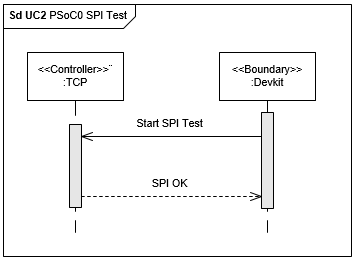
\includegraphics[width=.8\textwidth] {Systemarkitektur/images/SDPSoC0SPITest}
	\caption{Sekvensdiagram for PSoC0 SPI test}
	\label{fig:sekvensPSoC0SPITest}
\end{figure}

På figur \ref{fig:sekvensPSoC0SPITest} ses, at Devkittet sender en besked til kontrolklassen for at påbegynde SPI testen. Når testen er udført, svarer denne med en SPI OK og derved er SPI testen gennemført.

\begin{figure}[H]
	\centering
	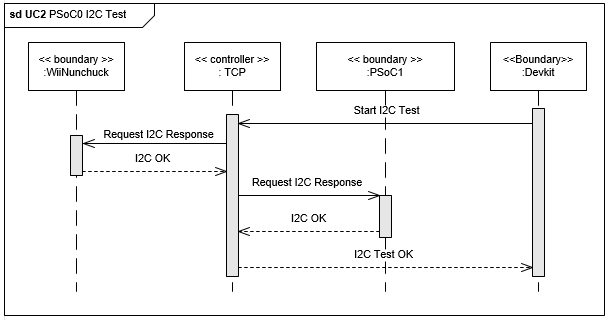
\includegraphics[width=\textwidth] {Systemarkitektur/images/SDPSoC0I2CTest}
	\caption{Sekvensdiagram for PSoC0 I2C test}
	\label{fig:sekvensPSoC0I2CTest}
\end{figure}

På figur \ref{fig:sekvensPSoC0I2CTest} ses, at Devkittet starter I2C testen, ved at sende en besked til kontroller klassen. Kontrolklassen anmoder herefter om svar via I2C nettet fra Nuchucken og PSoC1. Når disse enheder har svaret med et I2C OK er testen gennemført og der sendes besked til Devkittet med en I2C Test OK.

\begin{figure}[H]
	\centering
	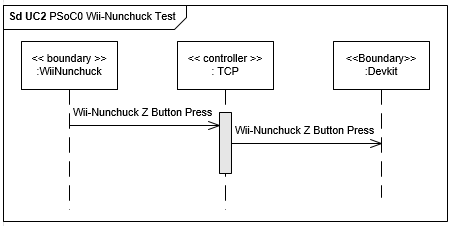
\includegraphics[width=\textwidth] {Systemarkitektur/images/SDPSoC0NunchuckTest}
	\caption{Sekvensdiagram for PSoC0 Nunchuck test}
	\label{fig:sekvensPSoC0NunchuckTest}
\end{figure}

På figur \ref{fig:sekvensPSoC0NunchuckTest} ses, at Nunchucken sender 'Z' knappens status (tryket eller ikke-trykket) til kontroller klassen. Denne videresender knappens status til Devkittet, og derved er testen færdig. \textbf{Devkit skal anmode om knaptryk på display. Ændres når SPI inkluderes}\newline

\begin{figure}[H]
	\centering
	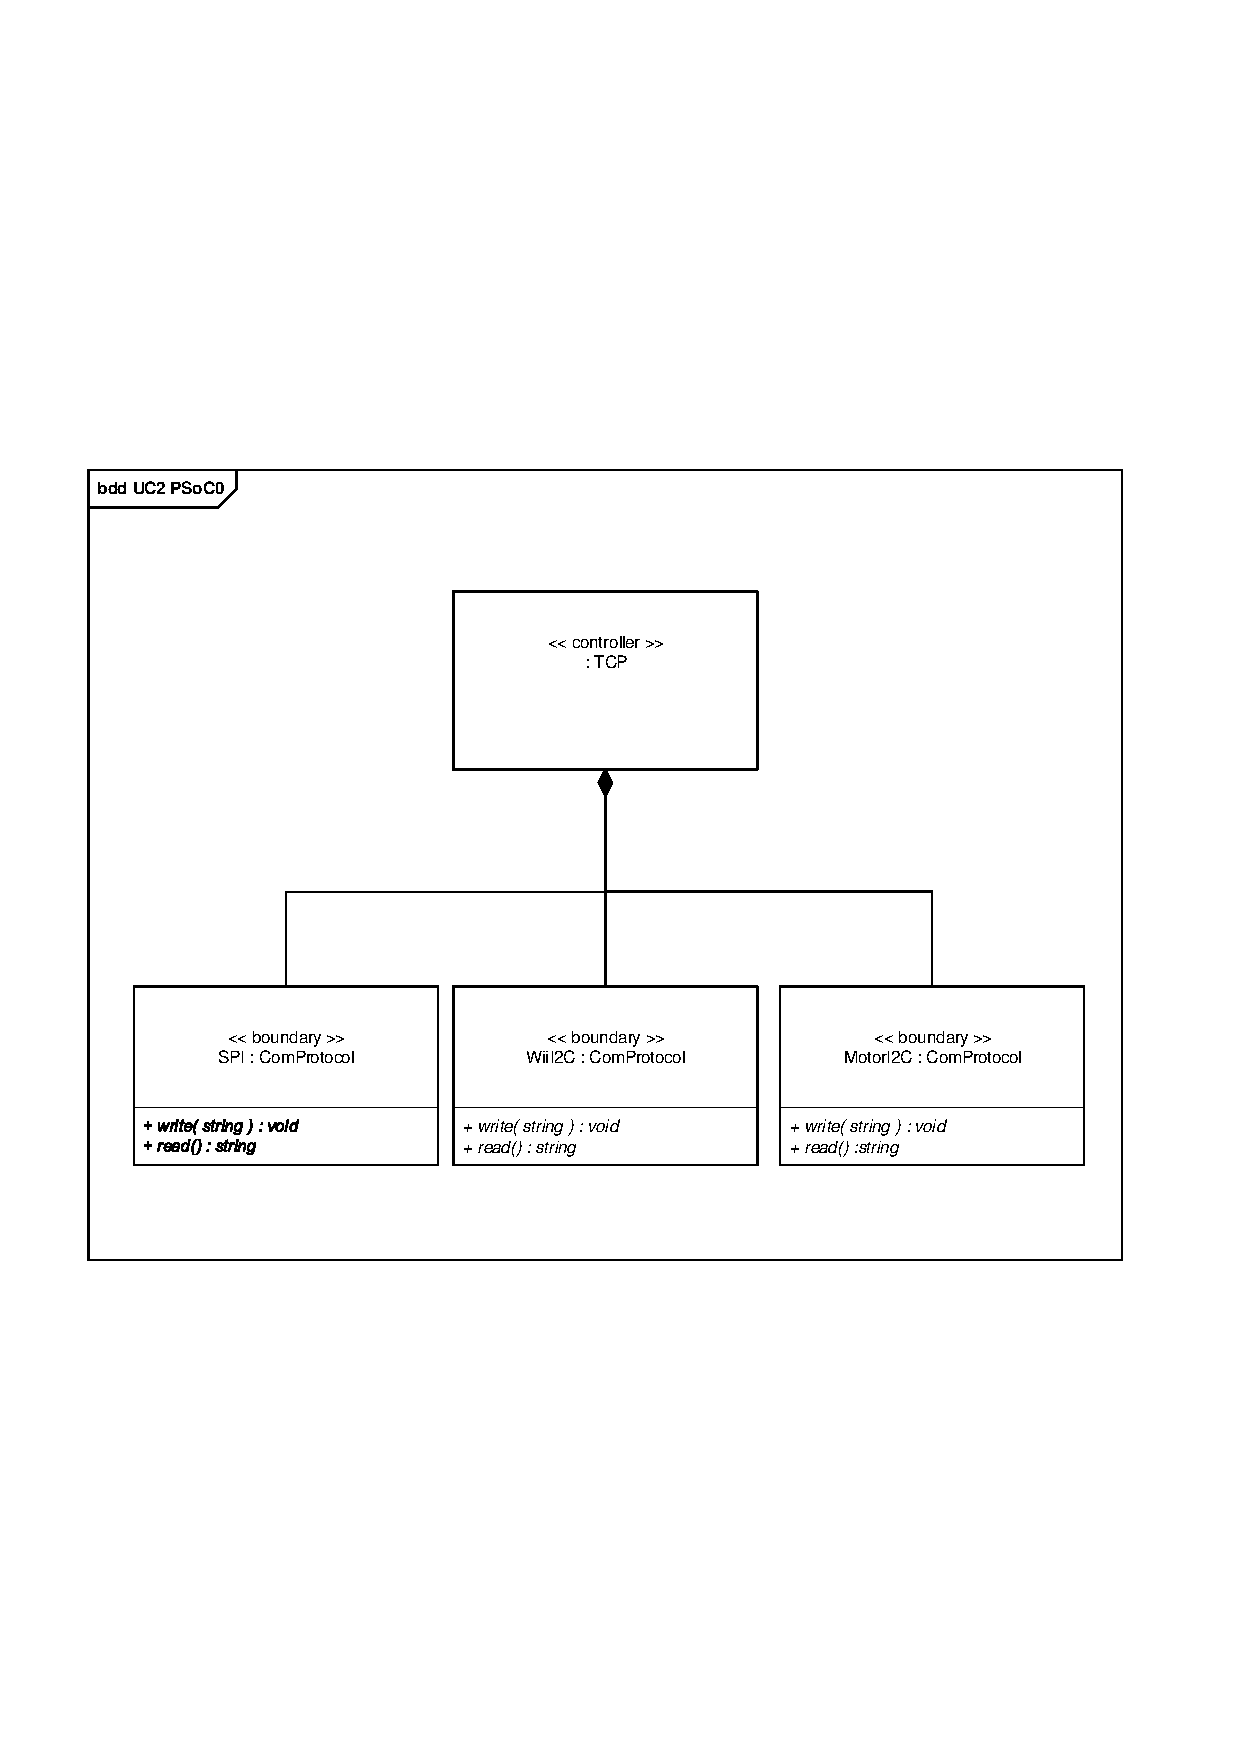
\includegraphics[width=\textwidth]{Systemarkitektur/images/klassediagramPSoC0}
	\caption{Klassediagram for PSoC0.}
	\label{fig:klassePSoC0}
\end{figure}

I klassediagrammet på figur \ref{fig:klassePSoC0} ses kontrolklassen og de tre boundaryklasser, som hører til PSoC0. I klasserne er der tilføjet metoder, som er udledt ud fra sekvensdiagrammerne. 

% ---------------PSoC1 Applikationsmodel-----------------------------
\subsection{Applikationsmodel for PSoC1}
Sekvensdiagrammet for PSoC1 ses på figur \ref{fig:sekvensPSoC1I2CTest}. Som forrig afsnit er kontrolklassen Test Communication Protocols, hvilket i diagrammet er forkortet til TCP. I dette tilfælde er der kun én boundaryklasse, da PSoC1, i denne use case, kun anvendes til I2C testen og derfor kun skal den kommunikere med PSoC0. 

\begin{figure}[H]
	\centering
	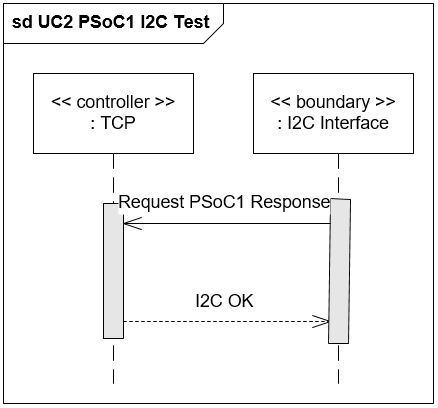
\includegraphics[width=.8\textwidth] {Systemarkitektur/images/SDPSoC1I2CTest}
	\caption{Sekvensdiagram for PSoC1}
	\label{fig:sekvensPSoC1I2CTest}
\end{figure}

På figur \ref{fig:sekvensPSoC1I2CTest} ses, at boundaryklassen anmoder om respons fra kontrolklassen til at bekræfte om at I2C slaven kan kommunikeres med. Hvis dette er tilfældet sendes der I2C OK tilbage til boundaryklassen.  

\begin{figure}[H]
	\centering
	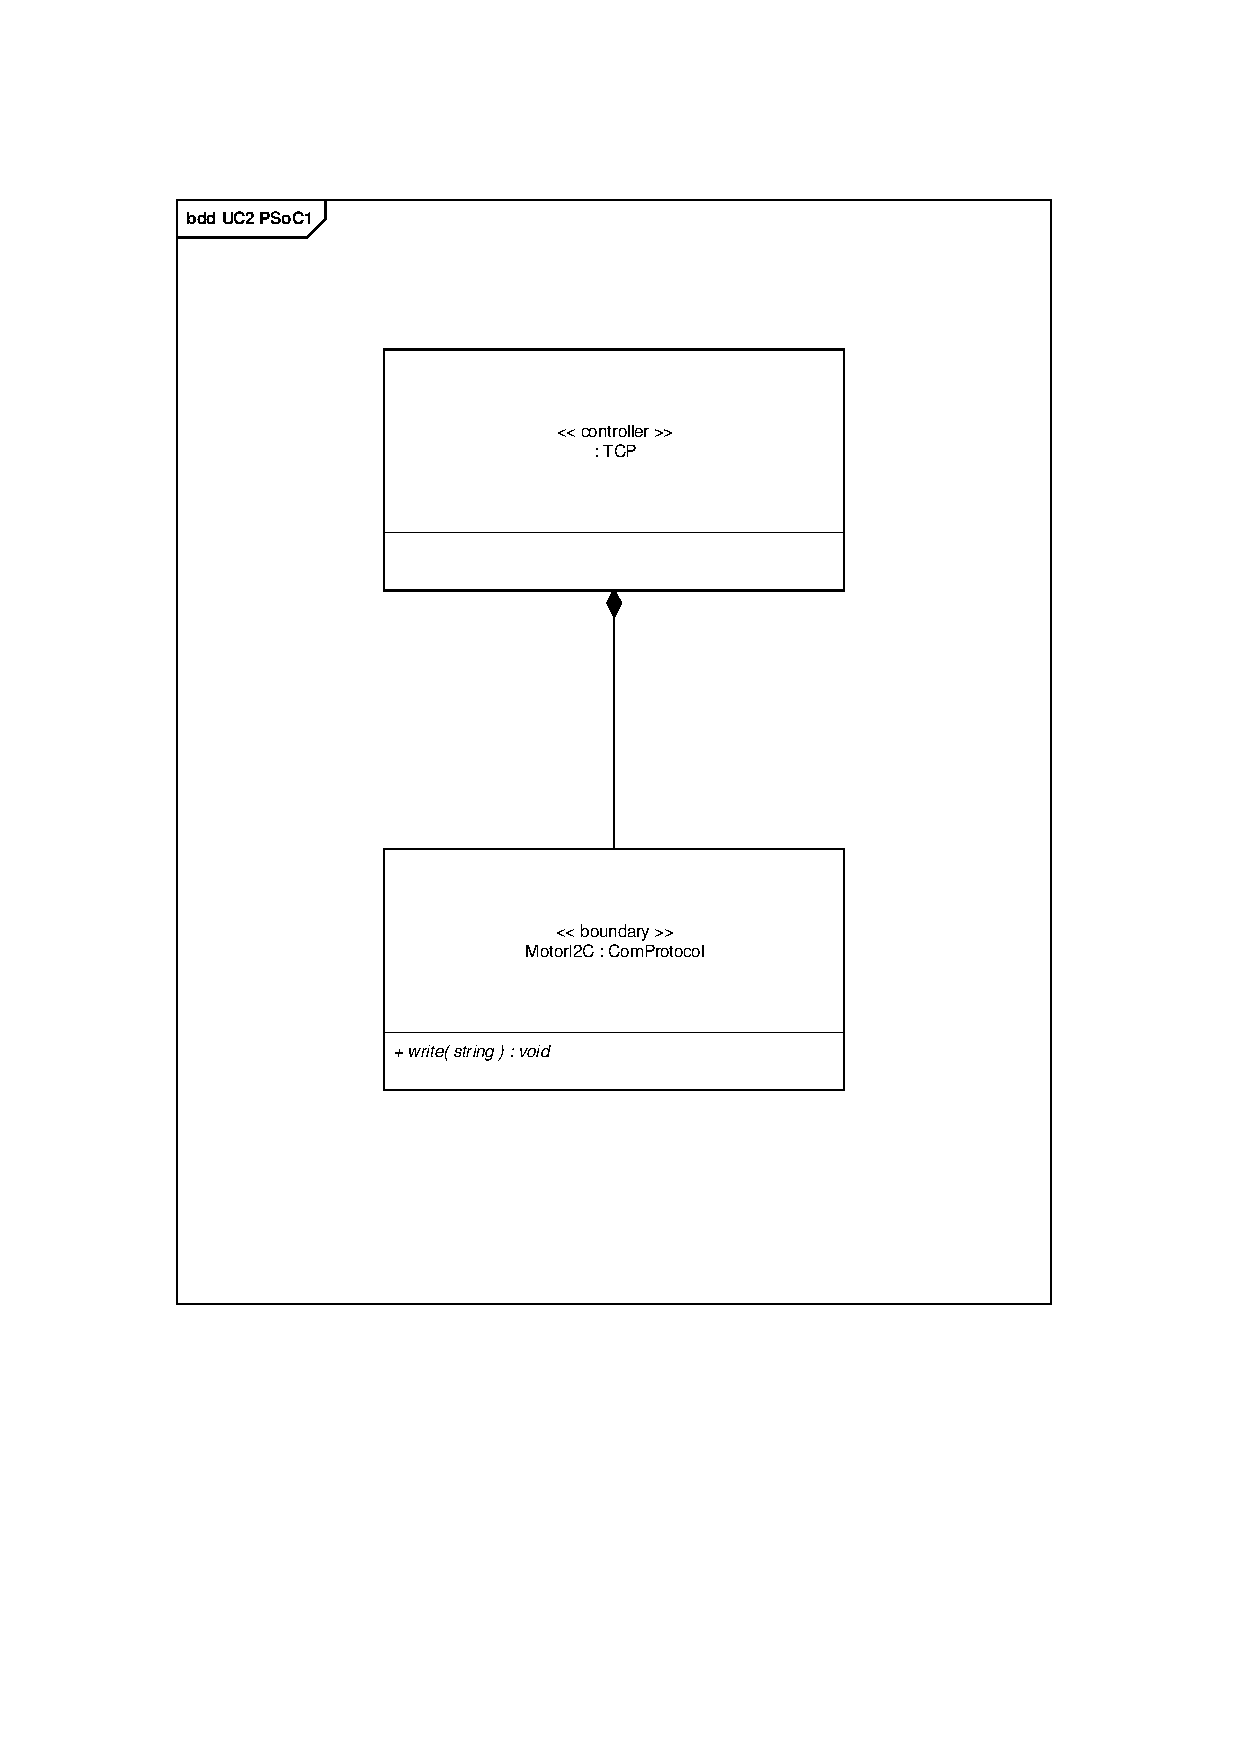
\includegraphics[width=.5\textwidth]{Systemarkitektur/images/klassediagramPSoC1}
	\caption{Klassediagram for PSoC1}
	\label{fig:klassePSoC1}
\end{figure}

Fra sekvensdiagrammet på figur \ref{fig:sekvensPSoC1I2CTest} udledes et klassediagram som ses foroven i figur \ref{fig:klassePSoC1}.

\subsection{Kommunikationsprotokoller}

I dette afsnit beskrives de kommunikationsprotokoller der anvendes til at sende data mellem systemets komponenter på de brugte bustyper - I2C og SPI.

På figur \ref{fig:kommunikationsOverblik} gives et overblik over forbindelserne mellem dets embedded linux platform og microcontrollers. Ved hver forbindelse ses typen af bus der bruges.

\begin{figure}[H]
	\centering
	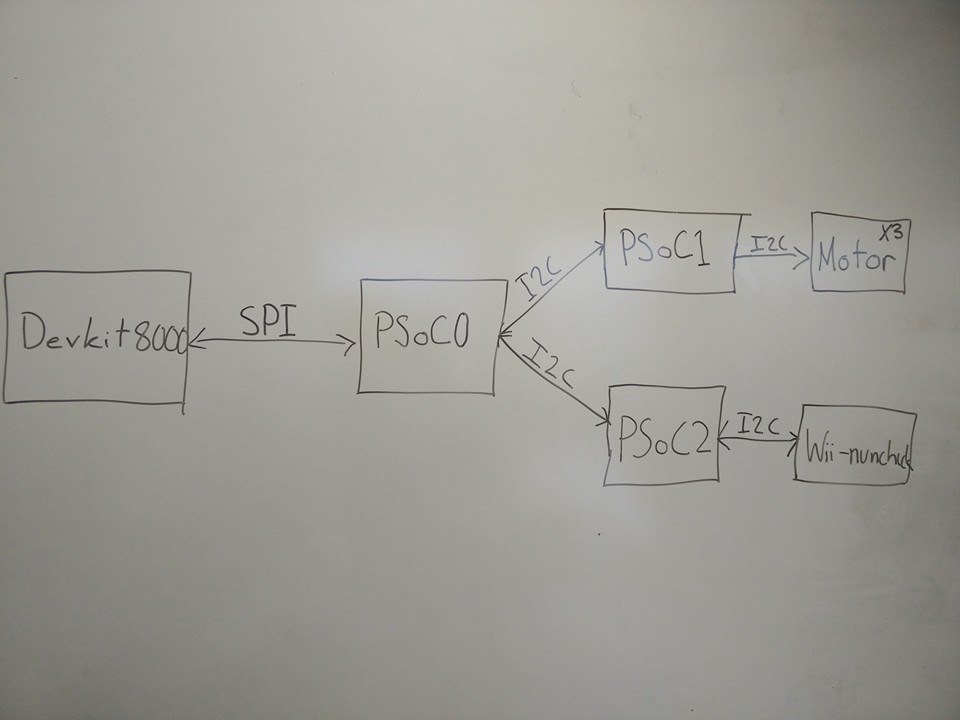
\includegraphics[width=\textwidth] {Systemarkitektur/images/overordnetstruktur}
	\caption{Forbindelser mellem systemets komponenter}
	\label{fig:kommunikationsOverblik}
\end{figure}

\subsubsection{SPI Protokol}

\subsubsection{I2C Protokol}
\label{afsnit:I2CProtokol}

I2C\cite{I2C} er en bus bestående af to ledninger. Den ene ledning bruges som databus og navngives \textit{Serial Data Line} (SDA). Den anden ledning bruges til clock signalet, til synkronisering kommunikationen, og navngives \textit{Serial Clock Line} (SCL). Enheder på I2C bussen gør brug af et master-slave forhold til at sende og læse data. En fordel ved I2C bussen er at netværket kan bestå af multiple masters og slaver, hvilket gavner sig godt for dette system da fire I2C komponenter skal sende data mellem hinanden.

I2C gør brug af en integreret protokol der anvender adressering af hardware-enheder for at identificere hvilken enhed der kommunikeres med. På tabel \ref{table:I2CAdress} ses addresserne tildelt systemets PSoCs.

\begin{table}[H]
	\centering
	\begin{tabular}{l|lllllll|l}
		\hline
		I2C Adresse bits & 7 & 6 & 5 & 4 & 3 & 2 & 1 & LSB er read/write indikator \\ \hline
		PSoC0        & 0 & 0 & 0 & 1 & 0 & 0 & 0 & 0/1                        \\
		PSoC1        & 0 & 0 & 0 & 1 & 0 & 0 & 1 & 0/1                        \\
		PSoC2        & 0 & 0 & 1 & 0 & 0 & 0 & 0 & 0/1                        \\ \hline
	\end{tabular}
	\caption{Adresser brugt på systemets I2C bus}
	\label{table:I2CAdress}
\end{table}

Den integrerede I2C protokol sender data serielt i pakker af 8-bit (1 byte). På figur \ref{fig:I2CTimingDiagram} ses et timing-diagram for aflæsning af 1 byte. Her ses at processen  begynder med en addresse-byte, efterfulgt af en data-byte. 

\begin{figure}[H]
	\centering
	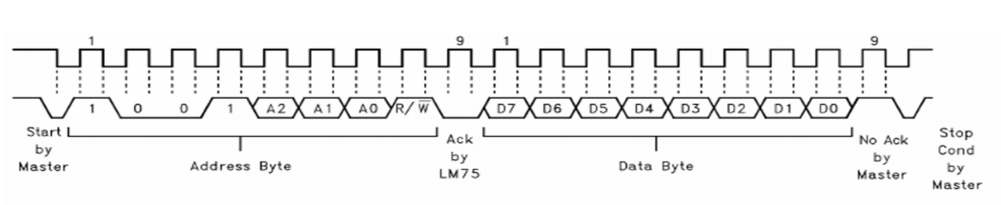
\includegraphics[width=\textwidth] {Systemarkitektur/images/I2CTimingDiagram}
	\caption{Timing Diagram af 1-byte I2C aflæsning}
	\label{fig:I2CTimingDiagram}
\end{figure}

Systemet gør brug af denne integrerede I2C protokol via en højere abstraheret \textit{Application Programming Interface} (API). Ved brug af denne API er en brugerdefineret protokol udviklet, som gør det muligt at sende kommandoer og data mellem systemets PSoC's.

Da I2C data udveksling - som beskrevet før - underliggende sker bytevist, er den brugerdefinerede I2C protokol opbygget ved at første modtagede byte indikerer typen af kommando. Herefter følger \textit{N} bytes som kommandoens tilhørende data. \textit{N} er et vilkårligt heltal og bruges i dette afsnit når der refereres til en mængde data-bytes der sendes med en kommandotype.

Modtagere bruger kommandoens type til at vide hvordan de efterfølgende data-bytes fortolkes. På figur \ref{fig:I2CProtokolEksempel} ses et sekvensdiagram der demonstrerer forløbet mellem en I2C afsender og modtager ved brug af I2C protokollen via pseudo-kommandoer.

\begin{figure}[H]
	\centering
	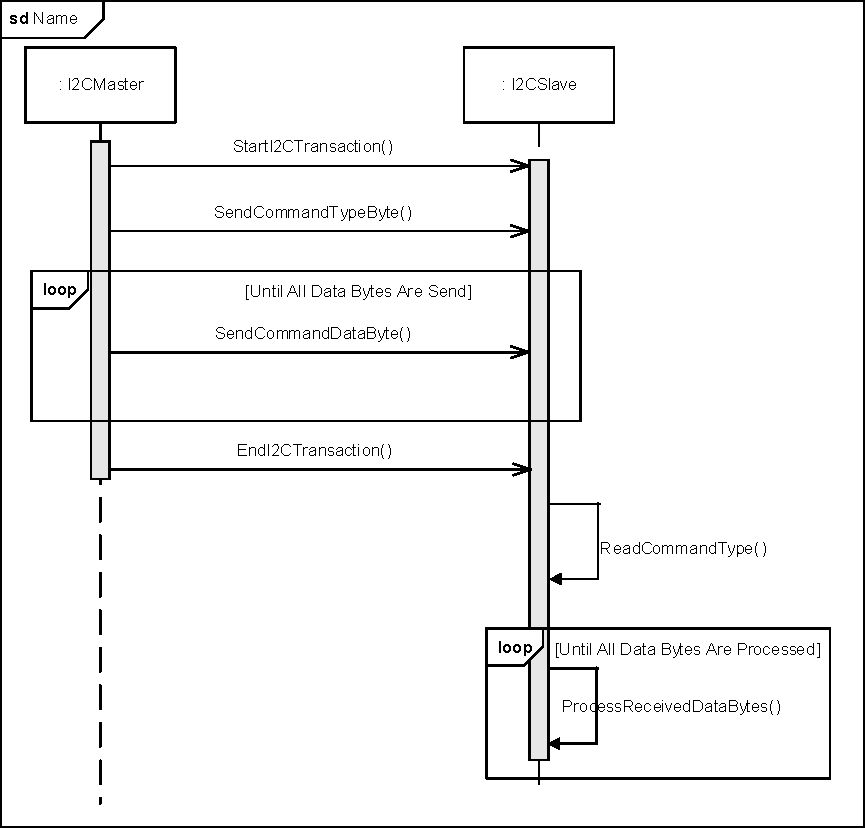
\includegraphics[width=\textwidth] {Systemarkitektur/images/I2CProtocol}
	\caption{Eksempel af I2C Protokol Forløb}
	\label{fig:I2CProtokolEksempel}
\end{figure}

Det kan på figur \ref{fig:I2CProtokolEksempel} ses at afsenderen først starter en I2C transaktion, hvorefter typen af kommando sendes som den første byte. Efterfølgende sendes \textit{N} antal bytes, afhængig af hvor meget data den givne kommandotype har brug for at sende. Efter afsluttet I2C transaktion læser I2C modtageren typen af kommando, hvor den herefter frit kan fortolke \textit{N} antal modtagne bytes afhængig af den modtagne kommandotype.

På tabel \ref{table:I2CKommandoer} ses de definerede kommandoer der gøres brug af.

\begin{table}[H]
	\centering
	\resizebox{\textwidth}{!}{%
		\begin{tabular}{lllll}
			\hline
			Kommando Type  & Beskrivelse                                           & Binær værdi & Hex værdi & Data bytes                                                                                                              \\ \hline
			\rowcolor[HTML]{EFEFEF} 
			NunchuckData   & Indeholder aflæst data fra Wii Nunchuck controlleren  & 0010 1010   & 0xA2      & \begin{tabular}[c]{@{}l@{}}Byte \#1 Analog X-værdi\\ Byte \#2 Analog Y-værdi\\ Byte \#3 Analog ButtonState\end{tabular} \\ \hline
			I2CTestRequest & Beder PSoC om at starte en I2C kommunikations test    & 0010 1001   & 0x29      & Ingen Databytes                                                                                                         \\ \hline
			\rowcolor[HTML]{EFEFEF} 
			I2CTestACK     & Beder om at få en I2C OK besked tilbage fra I2C enhed & 0010 1000   & 0x28      & Ingen Databytes                                                                                                         \\ \hline
		\end{tabular}%
	}
	\caption{De forskellige I2C Kommandoer der bruges}
	\label{table:I2CKommandoer}
\end{table}

Kolonnerne "Binær Værdi" og "Hex Værdi" i tabel \ref{table:I2CKommandoer} viser kommandotypens unikke tal-ID i både binær- og hexadecimalform. Det er denne værdi der sendes som den første byte, for at identificere kommandotypen. 




